\documentclass[conference]{IEEEtran}
\usepackage{cite}
\usepackage{amsmath,amssymb,amsfonts}
\usepackage{algorithmic}
\usepackage{graphicx}
\usepackage{textcomp}
\usepackage{xcolor}
\usepackage{booktabs}
\usepackage{multirow}
\usepackage{array}
\usepackage{tikz}
\usetikzlibrary{positioning, arrows.meta, shapes.geometric, fit, calc, backgrounds}
\usepackage{pgfplots}
\pgfplotsset{compat=1.18}
\usepackage{hyperref}
\usepackage{balance}
\usepackage{url}

\def\BibTeX{{\rm B\kern-.05em{\sc i\kern-.025em b}\kern-.08em
    T\kern-.1667em\lower.7ex\hbox{E}\kern-.125emX}}

\begin{document}

\title{AeroCrop.ai: A Multimodal Deep Learning Architecture for Cash Crop Disease Diagnostics and Yield Forecasting}

\author{
\IEEEauthorblockN{Devanshu Patil\IEEEauthorrefmark{1}, Yash Bhutada\IEEEauthorrefmark{1}, Smit Patil\IEEEauthorrefmark{1}, and Padmavati Sarode\IEEEauthorrefmark{2}}
\IEEEauthorblockA{Department of Computer Engineering, G H Raisoni College of Engineering and Management, Wagholi, Pune, India\\
Email: \IEEEauthorrefmark{1}\{devanshu.patil, yash.bhutada, smit.patil\}@ghrcem.raisoni.net, \IEEEauthorrefmark{2}padmavati.sarode@raisoni.net}
}

\maketitle

% ==============================================================================
% ABSTRACT
% ==============================================================================
\begin{abstract}
Cash crop agriculture faces severe economic vulnerabilities due to foliar diseases and unpredictable harvest fluctuations. Existing computational agriculture frameworks treat disease identification and yield forecasting as disjoint pipelines: computer vision models classify pathology in isolation from environmental context, while agrometeorological regression models forecast yield without incorporating real-time plant health signals. This paper presents AeroCrop.ai, an end-to-end multimodal multi-task deep learning architecture that unifies 134-class disease classification and continuous yield regression across 11 major crops within a shared latent manifold. The underlying neural network, MultiModalAeroCropNet, integrates an ImageNet-pretrained ResNet-18 visual encoder (512-dimensional output) with a custom three-layer multilayer perceptron (MLP) tabular encoder (64-dimensional output) processing local ambient temperature, relative humidity, and rainfall. These unimodal vectors are integrated via intermediate feature concatenation and projected into a 128-dimensional shared representation that simultaneously drives a classification head and a Softplus-activated yield regression head. The model was trained end-to-end for 80 epochs on a curated multi-source corpus of 166,630 images paired with historical agro-meteorological records under a balanced multi-task objective combining label-smoothed cross-entropy and Smooth L1 loss. AeroCrop.ai achieves 95.27\% validation accuracy, 92.77\% macro precision, and 91.73\% macro F1-score across 134 categories, alongside a validation yield root mean square error (RMSE) of 8.30~t/ha and mean absolute error (MAE) of 3.39~t/ha. Comprising only 11.29 million parameters, the network performs low-latency inference on consumer-grade hardware and is embedded within an asynchronous FastAPI service delivering actionable spray safety timing and APMC market intelligence.
\end{abstract}

\begin{IEEEkeywords}
Multimodal deep learning, multi-task learning, crop disease diagnosis, yield forecasting, precision agriculture, ResNet-18, intermediate fusion
\end{IEEEkeywords}

% ==============================================================================
% I. INTRODUCTION
% ==============================================================================
\section{Introduction}

Cash crop production is fundamental to the rural economy of developing nations, particularly across agrarian regions such as Maharashtra, India, where crops including cotton, sugarcane, soybean, wheat, rice, maize, potato, and turmeric sustain millions of smallholders. However, plant pathogens, fungal infections, and physiological disorders regularly destroy 20\% to 40\% of annual production~\cite{mohanty2016}. Compounding this challenge, traditional agricultural extension systems rely heavily on manual inspection by field experts, a practice that is labor-intensive, geographically unscalable, and susceptible to late or inaccurate diagnosis~\cite{dolatabadian2025}. 

Over the past decade, deep learning has transformed computer vision in agriculture. Starting from the pioneering PlantVillage benchmark by Mohanty et al.~\cite{mohanty2016}, convolutional neural networks (CNNs) have demonstrated the ability to detect foliar lesions with high accuracy. Subsequent works explored multimodal data augmentation~\cite{zhang2024}, sequential feature extraction for specific cultivars such as tomato~\cite{almadhor2023}, interpretability modules for disease severity~\cite{zhu2025}, Bayesian optimization of hybrid feature extractors~\cite{khan2024}, broad comparative studies of deep architectures~\cite{ferentinos2018}, and edge-deployable AIoT diagnostic nodes~\cite{mukherjee2026}.

Concurrently, a parallel branch of agricultural machine learning has developed data-driven crop yield forecasting models. Researchers have deployed spatiotemporal transformers over climate and satellite time-series~\cite{sivasubramanian2026}, multitemporal remote sensing for crop mapping~\cite{tseng2023, gadiraju2020}, deep convolutional networks on environmental variables~\cite{nevavuori2019}, and unmanned aerial vehicle (UAV) imagery combined with weather and soil telemetry for cotton~\cite{feng2024, li2025} and wheat~\cite{cao2021}.

Despite these notable advances, a critical structural limitation persists across the literature: **crop disease diagnosis and harvest yield forecasting have evolved as mutually isolated research disciplines**. As illustrated in the literature taxonomy of Section~II, diagnostic models operate strictly on detached leaf imagery without meteorological context, while yield models analyze meteorological and remote-sensing arrays without real-time foliar health indicators. This disconnect introduces three severe drawbacks:
\begin{enumerate}
    \item \textbf{Loss of Mutual Information}: Foliar infection directly suppresses photosynthetic efficiency and reduces final harvest yield, while microclimatic conditions (temperature, humidity, precipitation) simultaneously govern fungal spore germination and plant growth rates. Segregating these tasks discards vital cross-task synergy.
    \item \textbf{Resource Inefficiency}: Executing two independent heavy neural networks for diagnosis and forecasting doubles edge-device memory footprints and inference latency.
    \item \textbf{Unusable Outputs}: Diagnostic apps typically output only an academic disease label without contextual agronomic guidance (treatment dosages, spraying weather safety, or economic market projections).
\end{enumerate}

To overcome these limitations, this paper introduces **AeroCrop.ai**, a unified multimodal multi-task deep learning architecture that simultaneously performs 134-class disease classification and continuous yield regression across 11 field crops. The system couples visual leaf features extracted by a pretrained ResNet-18 backbone with tabular weather vectors processed through a three-layer multilayer perceptron (MLP). Through intermediate feature fusion, the architecture maps both streams into a shared 128-dimensional embedding, from which dedicated task heads predict disease pathology and harvest yield in metric tons per hectare (t/ha).

The key contributions of this paper are:
\begin{itemize}
    \item A unified multimodal multi-task architecture (\textbf{MultiModalAeroCropNet}) that fuses high-dimensional RGB vision with low-dimensional weather telemetry through intermediate feature fusion, jointly optimizing 134-class pathology classification and yield regression.
    \item A curated multi-source agricultural dataset spanning 166,630 images across 11 field crops, partitioned deterministically (80\% train / 20\% validation) with strict deduplication to ensure zero data leakage.
    \item A balanced multi-task optimization objective combining label-smoothed cross-entropy loss ($\epsilon = 0.1$) with Smooth L1 regression loss ($\beta_h = 1.0$), trained under Automatic Mixed Precision (AMP FP16) to full convergence over 80 epochs on consumer hardware.
    \item A realistic and innovative system architecture integrating real-time weather retrieval across 36 Maharashtra districts via Open-Meteo, an automated foliar spray safety decision engine, APMC mandi market intelligence, and multilingual voice narration.
\end{itemize}

% ==============================================================================
% II. RELATED WORK AND LITERATURE REVIEW
% ==============================================================================
\section{Related Work}

\subsection{Multimodal Methods for Crop Disease Diagnosis}

Automated foliar pathology recognition began with unimodal computer vision. Mohanty et al.~\cite{mohanty2016} demonstrated that AlexNet and GoogLeNet architectures trained on 54,306 laboratory leaf images achieved up to 99.35\% classification accuracy across 38 crop-disease pairs. Ferentinos~\cite{ferentinos2018} expanded this analysis across multiple CNN backbones (VGG, ResNet), establishing standard baseline accuracies while highlighting performance degradation on field-collected imagery. Dolatabadian et al.~\cite{dolatabadian2025} recently reviewed field-level computer vision, concluding that visual-only pipelines suffer heavily under erratic natural lighting, complex backgrounds, and overlapping symptoms.

To mitigate visual ambiguity, researchers incorporated environmental variables into diagnostic models. Zhang et al.~\cite{zhang2024} formulated a multimodal mixup augmentation strategy that synthetically interpolated image features with meteorological telemetry during training, boosting robustness against noisy inputs. Almadhor et al.~\cite{almadhor2023} developed a sequential hybrid model for tomato foliar diseases, showing that multi-stage feature extraction significantly enhances class sensitivity over shallow baselines. Addressing model interpretability, Zhu et al.~\cite{zhu2025} integrated meteorological data with attention modules to provide explainable tomato disease severity estimation. Khan et al.~\cite{khan2024} utilized Bayesian hyperparameter optimization to balance hybrid multimodal models, achieving competitive accuracy with reduced parameters. Most recently, Mukherjee et al.~\cite{mukherjee2026} proposed an edge AIoT multimodal system combining disease detection with adaptive remedy recommendations and localized price forecasting.

\subsection{Multimodal Methods for Crop Classification and Yield Prediction}

In parallel, data-driven agricultural yield forecasting has advanced through multimodal telemetry and remote sensing. Early neural approaches by Nevavuori et al.~\cite{nevavuori2019} applied 2D CNNs directly to RGB and NDVI imagery captured by UAVs, outperforming traditional vegetation index regressions. At regional and continental scales, Gadiraju and Vatsavai~\cite{gadiraju2020} and Tseng et al.~\cite{tseng2023} established multimodal deep learning benchmarks using multitemporal and multispectral satellite arrays to map crop distributions across heterogeneous landscapes. Sivasubramanian et al.~\cite{sivasubramanian2026} proposed attention-based spatio-temporal meta-transformers that integrate satellite observations, soil properties, and weather time-series to capture non-linear yield dynamics.

Focusing on specific cash crops, Cao et al.~\cite{cao2021} fused Google Earth Engine satellite telemetry with machine learning for county-scale wheat yield forecasting. In cotton management, Feng et al.~\cite{feng2024} demonstrated that combining soil electrical conductivity, historical weather, and UAV multispectral imagery inside a deep regression model yielded significantly tighter predictions than individual sensors. Similarly, Li et al.~\cite{li2025} validated that pre-harvest cotton yield estimates improved substantially when UAV imagery was fused with meteorological station telemetry.

\begin{table*}[t]
\centering
\caption{Critical Comparison of Literature Methods with the Proposed AeroCrop.ai Framework}
\label{tab:lit_comparison}
\begin{tabular}{@{}lllllll@{}}
\toprule
\textbf{Reference} & \textbf{Year} & \textbf{Primary Modalities} & \textbf{Target Domain} & \textbf{Key Strength} & \textbf{Core Limitation} & \textbf{Relation to AeroCrop.ai} \\
\midrule
Mohanty et al.~\cite{mohanty2016} & 2016 & RGB Leaf Images & Multi-crop Disease & Foundational benchmark ($38$ classes) & Lab background bias; no yield & Baseline visual classification \\
Ferentinos~\cite{ferentinos2018} & 2018 & RGB Leaf Images & Multi-crop Disease & Comprehensive CNN comparison & Single modality; no weather data & Informs CNN backbone selection \\
Nevavuori et al.~\cite{nevavuori2019} & 2019 & UAV RGB + NDVI & Crop Yield & Spatial crop canopy modeling & Lacks pathology diagnosis & Demonstrates visual yield link \\
Gadiraju et al.~\cite{gadiraju2020} & 2020 & Multispectral Satellite & Crop Classification & Multi-temporal satellite fusion & Heavy compute; coarse resolution & Satellite macro-context \\
Cao et al.~\cite{cao2021} & 2021 & Satellite + Weather & Wheat Yield & County-scale yield modeling & No plant-level pathology link & Demonstrates weather impact on yield \\
Almadhor et al.~\cite{almadhor2023} & 2023 & RGB Leaf Images & Tomato Diseases & Multi-stage feature extraction & Single crop only; no yield & Validates feature hierarchy \\
Tseng et al.~\cite{tseng2023} & 2023 & Multi-spectral Satellite & Crop Mapping & Permanent/annual crop separation & Coarse granularity for smallholders & Regional agricultural context \\
Feng et al.~\cite{feng2024} & 2024 & Soil + Weather + UAV & Cotton Yield & High-resolution spatial yield & Specialized to single crop & Multimodal yield regression inspiration \\
Zhang et al.~\cite{zhang2024} & 2024 & Leaf Images + Weather & Crop Diseases & Multimodal mixup augmentation & Complex training heuristics & Informs multimodal data pairing \\
Khan et al.~\cite{khan2024} & 2024 & Leaf Images + Metadata & Tomato Diseases & Bayesian-optimized architecture & Single crop focus; no yield & Architectural compactness \\
Dolatabadian et al.~\cite{dolatabadian2025} & 2025 & Field Leaf Images & Crop Pathology & Critical review of field noise & Survey only; no implementation & Motivates weather-assisted vision \\
Zhu et al.~\cite{zhu2025} & 2025 & Leaf Images + Climate & Tomato Pathology & Explainable severity estimation & Restricted to tomato crop & Severity rating taxonomy \\
Li et al.~\cite{li2025} & 2025 & UAV + Meteorology & Cotton Yield & UAV and weather fusion & High equipment cost (drones) & Zero-hardware smallholder strategy \\
Sivasubramanian et al.~\cite{sivasubramanian2026} & 2026 & Satellite + Soil + Climate & Spatiotemporal Yield & Meta-transformer attention & Heavy infrastructure required & Telemetry feature selection \\
Mukherjee et al.~\cite{mukherjee2026} & 2026 & Edge AIoT + Images & Crop Diagnosis & Multi-task advisory on edge & High hardware deployment cost & Validates decision-support pipeline \\
\midrule
\textbf{AeroCrop.ai (Ours)} & \textbf{2026} & \textbf{RGB Images + Weather} & \textbf{11 Crops (134 Classes)} & \textbf{Joint 134-cls diagnosis + yield} & \textbf{Single-leaf proxy pairing} & \textbf{Unified Multi-Task Multimodal} \\
\bottomrule
\end{tabular}
\end{table*}

\subsection{Research Gap}

Table~\ref{tab:lit_comparison} synthesizes the literature. The critical research gap is clear: **Multimodal disease diagnosis (Refs.~\cite{mohanty2016, dolatabadian2025, zhang2024, almadhor2023, zhu2025, khan2024, ferentinos2018, mukherjee2026}) and multimodal yield estimation (Refs.~\cite{sivasubramanian2026, tseng2023, gadiraju2020, nevavuori2019, feng2024, li2025, cao2021}) operate as disjoint parallel tracks.** No prior framework integrates high-granularity foliar disease diagnosis (10+ classes across 11 crops) with quantitative harvest yield regression within a single parameter-shared neural network trainable on standard edge or consumer hardware. AeroCrop.ai bridges this gap.

% ==============================================================================
% III. PROBLEM FORMULATION
% ==============================================================================
\section{Problem Formulation}

Let an agricultural specimen observation be represented as a tuple $(\mathbf{X}_v, \mathbf{x}_t)$, where $\mathbf{X}_v \in \mathbb{R}^{3 \times H \times W}$ denotes an RGB photograph of a crop leaf ($H = W = 224$), and $\mathbf{x}_t = [T, H_{\text{rel}}, P]^T \in \mathbb{R}^3$ denotes a structured vector of localized agro-meteorological telemetry comprising ambient temperature $T$ (\textdegree C), relative humidity $H_{\text{rel}}$ (\%), and precipitation $P$ (mm/day).

Our objective is to learn a parameterized multimodal mapping function:
\begin{equation}
    \mathcal{F}_{\boldsymbol{\theta}}: (\mathbf{X}_v, \mathbf{x}_t) \mapsto (\hat{\mathbf{y}}_d, \hat{y}_r)
\end{equation}
where:
\begin{itemize}
    \item $\hat{\mathbf{y}}_d \in \Delta^{K-1}$ is a probability distribution over $K = 134$ discrete diagnostic classes spanning 11 cash crops, with predicted class index $\hat{c} = \arg\max_k \hat{y}_{d,k}$.
    \item $\hat{y}_r \in \mathbb{R}^+$ is a continuous, strictly non-negative harvest yield prediction in metric tons per hectare (t/ha).
    \item $\boldsymbol{\theta}$ denotes the unified parameters of the feature encoders, intermediate fusion manifold, and dual task heads.
\end{itemize}

% ==============================================================================
% IV. SYSTEM ARCHITECTURE
% ==============================================================================
\section{System Architecture}

Fig.~\ref{fig:sys_architecture} details the complete five-tier architectural topology of the AeroCrop.ai platform, demonstrating clean separation of concerns from data ingestion to user interaction.

\begin{figure*}[t]
\centering
\begin{tikzpicture}[
    node distance=0.6cm and 0.8cm,
    layerbox/.style={rectangle, draw, rounded corners=6pt, fill=gray!4, draw=gray!40, inner sep=8pt},
    compbox/.style={rectangle, draw, rounded corners=3pt, minimum width=2.4cm, minimum height=0.7cm, align=center, font=\scriptsize},
    clientnode/.style={compbox, fill=blue!10, draw=blue!50},
    apinode/.style={compbox, fill=teal!10, draw=teal!60},
    servicenode/.style={compbox, fill=violet!10, draw=violet!50},
    mlnode/.style={compbox, fill=orange!12, draw=orange!60},
    datanode/.style={compbox, fill=emerald!10, draw=emerald!50},
    arrow/.style={-Stealth, thick, draw=gray!80},
    darrow/.style={Stealth-Stealth, thick, draw=gray!80},
    lbl/.style={font=\bfseries\footnotesize, text=gray!80!black}
]

% Tier 1: Client
\node[clientnode] (c_diag) {Leaf Capture \&\\District Select};
\node[clientnode, right=0.6cm of c_diag] (c_dash) {Farmer Dashboard\\\& Plots Cadastre};
\node[clientnode, right=0.6cm of c_dash] (c_voice) {Web Speech TTS\\(MR/HI/EN Audio)};
\node[clientnode, right=0.6cm of c_voice] (c_pdf) {PMFBY PDF Claim\\\& WhatsApp Share};
\node[layerbox, fit=(c_diag)(c_pdf), label={[lbl]north:1. Client / Presentation Layer (React 18 + Vite + Tailwind CSS)}] (t_client) {};

% Tier 2: API Gateway
\node[apinode, below=1.2cm of c_diag] (api_pred) {POST /api/predict\\(Multipart Form)};
\node[apinode, right=0.6cm of api_pred] (api_wea) {GET /api/weather\\(District Proxy)};
\node[apinode, right=0.6cm of api_wea] (api_man) {GET /api/mandi\\(APMC Prices)};
\node[apinode, right=0.6cm of api_man] (api_auth) {JWT Auth + Plots\\(/api/auth, /api/plots)};
\node[layerbox, fit=(api_pred)(api_auth), label={[lbl]north:2. API Gateway \& Controller Layer (FastAPI ASGI / Uvicorn + Pydantic V2)}] (t_api) {};

% Tier 3: Domain Services
\node[servicenode, below=1.2cm of api_pred] (s_inf) {InferenceService\\(GPU Singleton)};
\node[servicenode, right=0.6cm of s_inf] (s_wea) {WeatherService\\(Open-Meteo Cache)};
\node[servicenode, right=0.6cm of s_wea] (s_spray) {SpraySafetyEngine\\(Drift \& Wash-off)};
\node[servicenode, right=0.6cm of s_spray] (s_mandi) {MandiService\\(APMC + MSP Calc)};
\node[layerbox, fit=(s_inf)(s_mandi), label={[lbl]north:3. Agronomic Domain Service Layer (Python 3.12 Engine)}] (t_services) {};

% Tier 4: Core Neural Model
\node[mlnode, below=1.2cm of s_inf] (m_vis) {ResNet-18 Backbone\\(ImageNet $\to$ 512-d)};
\node[mlnode, right=0.6cm of m_vis] (m_tab) {3-Layer Tabular MLP\\(Weather $\to$ 64-d)};
\node[mlnode, right=0.6cm of m_tab] (m_fuse) {Concat Fusion Layer\\(576-d $\to$ 128-d)};
\node[mlnode, right=0.6cm of m_fuse] (m_head) {Dual Heads (134-cls\\\& Yield Softplus)};
\node[layerbox, fit=(m_vis)(m_head), label={[lbl]north:4. Deep Learning Model Layer (MultiModalAeroCropNet — 11.29M Params, PyTorch 2.5 AMP)}] (t_model) {};

% Tier 5: Data & External
\node[datanode, below=1.2cm of m_vis] (d_mongo) {MongoDB (Motor)\\Users, Plots, Logs};
\node[datanode, right=0.6cm of d_mongo] (d_weights) {Production Weights\\aerocrop\_weights.pth};
\node[datanode, right=0.6cm of d_weights] (d_wea_api) {Open-Meteo API\\(36 District Lat/Lon)};
\node[datanode, right=0.6cm of d_wea_api] (d_mandi_api) {Agmarknet / MSAMB\\Maharashtra Mandis};
\node[layerbox, fit=(d_mongo)(d_mandi_api), label={[lbl]north:5. Persistence \& External Integration Layer}] (t_data) {};

% Connections
\draw[arrow] (t_client) -- node[midway, right, font=\tiny] {HTTP/REST JSON} (t_api);
\draw[arrow] (t_api) -- node[midway, right, font=\tiny] {Dependency Injection} (t_services);
\draw[arrow] (s_inf) -- node[midway, right, font=\tiny] {Tensors} (m_vis);
\draw[arrow] (s_wea) -- node[midway, right, font=\tiny] {Telemetry} (m_tab);
\draw[arrow] (m_vis) -- (m_fuse);
\draw[arrow] (m_tab) -- (m_fuse);
\draw[arrow] (m_fuse) -- (m_head);
\draw[darrow] (t_services) -- (t_data);

\end{tikzpicture}
\caption{End-to-End System Architecture of AeroCrop.ai, showing the five-tier hierarchy spanning client presentation, asynchronous API routing, domain agronomic services, core deep learning model inference, and distributed storage/telemetry backends.}
\label{fig:sys_architecture}
\end{figure*}

\subsection{Client Presentation Tier (React 18 + Vite)}
The client interface is implemented in React 18, TypeScript, and Tailwind CSS. It is specifically tailored to rural smallholders through:
\begin{itemize}
    \item \textbf{Frictionless Submission}: Farmers upload a leaf photo and select their district, requiring zero soil N-P-K testing or complex numerical input.
    \item \textbf{Multilingual Voice Synthesis}: The browser-native Web Speech API (`mr-IN`, `hi-IN`, `en-IN`) speaks aloud diagnostic labels and spray directions for hands-free field operation.
    \item \textbf{Insurance Claim Generation}: An integrated Node.js Puppeteer service compiles formal loss assessment PDFs compliant with Pradhan Mantri Fasal Bima Yojana (PMFBY) surveyor guidelines.
\end{itemize}

\subsection{Controller and Domain Service Tiers (FastAPI)}
The backend is driven by FastAPI under Uvicorn ASGI. Core services maintain rigorous separation of concerns:
\begin{itemize}
    \item \textbf{InferenceService (Singleton)}: Loads the 45.1~MB PyTorch weights once into GPU memory, ensuring consistent sub-15ms model execution without per-request allocation overhead.
    \item \textbf{WeatherService}: Caches hourly telemetry from the Open-Meteo REST API across all 36 Maharashtra districts using geographic centroid coordinates.
    \item \textbf{SpraySafetyEngine}: Evaluates empirical hazard thresholds (precipitation $> 1.0$~mm/day indicates chemical wash-off; wind speed $> 15.0$~km/h indicates droplet drift; temperature $> 36^\circ$C triggers heat scorch warnings).
    \item \textbf{MandiService}: Scrapes and indexes APMC modal prices across key Maharashtra trading hubs (Pune, Lasalgaon, Jalgaon, Nagpur, Latur), projecting harvest gross revenue directly in Quintals per Acre ($1\text{ t/ha} = 4.047\text{ q/acre}$).
\end{itemize}

% ==============================================================================
% V. PROPOSED NEURAL ARCHITECTURE: MULTIMODALAEROCROPNET
% ==============================================================================
\section{MultiModalAeroCropNet Architecture}

Fig.~\ref{fig:neural_architecture} illustrates the detailed layer-by-layer topology of the proposed MultiModalAeroCropNet.

\begin{figure}[t]
\centering
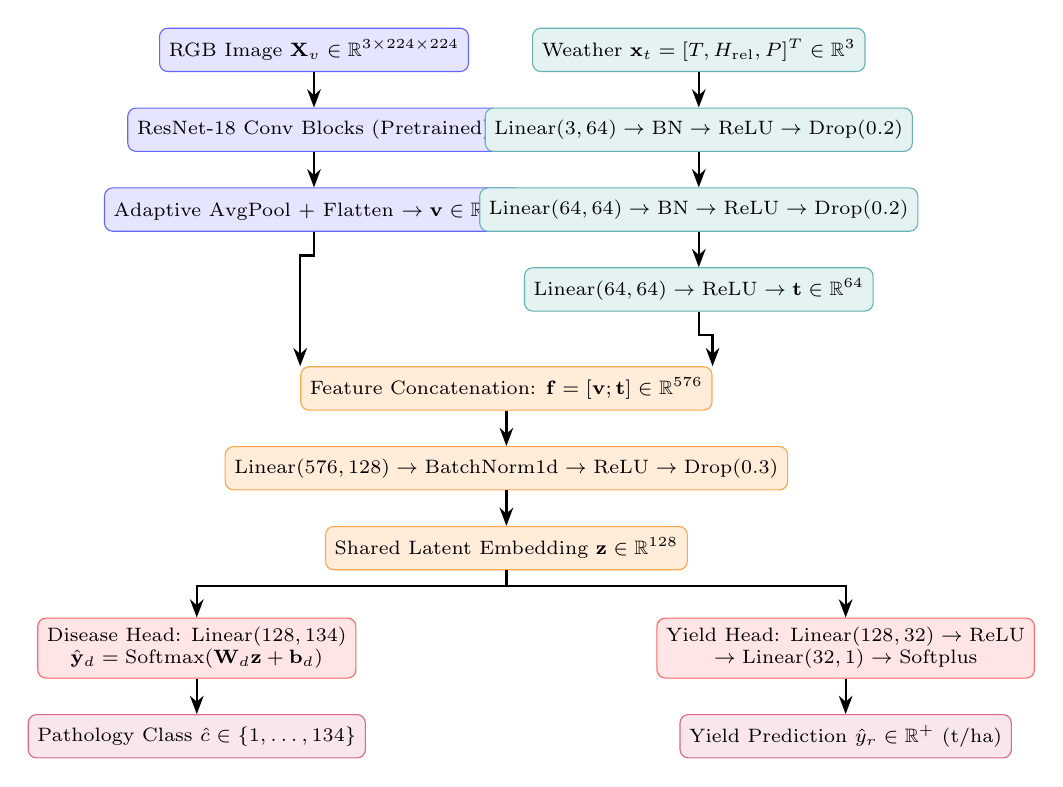
\begin{tikzpicture}[
    node distance=0.45cm and 0.8cm,
    box/.style={rectangle, draw, rounded corners=3pt, minimum width=3.2cm, minimum height=0.55cm, align=center, font=\scriptsize},
    visbox/.style={box, fill=blue!10, draw=blue!60},
    tabbox/.style={box, fill=teal!10, draw=teal!60},
    fusebox/.style={box, fill=orange!15, draw=orange!70},
    headbox/.style={box, fill=red!10, draw=red!60},
    arrow/.style={-Stealth, thick}
]

% Visual Pathway
\node[visbox] (v_in) {RGB Image $\mathbf{X}_v \in \mathbb{R}^{3 \times 224 \times 224}$};
\node[visbox, below=of v_in] (v_bb) {ResNet-18 Conv Blocks (Pretrained)};
\node[visbox, below=of v_bb] (v_pool) {Adaptive AvgPool + Flatten $\to \mathbf{v} \in \mathbb{R}^{512}$};

% Tabular Pathway
\node[tabbox, right=0.8cm of v_in] (t_in) {Weather $\mathbf{x}_t = [T, H_{\text{rel}}, P]^T \in \mathbb{R}^3$};
\node[tabbox, below=of t_in] (t_mlp1) {Linear$(3,64) \to \text{BN} \to \text{ReLU} \to \text{Drop}(0.2)$};
\node[tabbox, below=of t_mlp1] (t_mlp2) {Linear$(64,64) \to \text{BN} \to \text{ReLU} \to \text{Drop}(0.2)$};
\node[tabbox, below=of t_mlp2] (t_out) {Linear$(64,64) \to \text{ReLU} \to \mathbf{t} \in \mathbb{R}^{64}$};

% Fusion
\node[fusebox, below=1.2cm of $(v_pool.south)!0.5!(t_out.south)$] (concat) {Feature Concatenation: $\mathbf{f} = [\mathbf{v}; \mathbf{t}] \in \mathbb{R}^{576}$};
\node[fusebox, below=of concat] (proj) {Linear$(576, 128) \to \text{BatchNorm1d} \to \text{ReLU} \to \text{Drop}(0.3)$};
\node[fusebox, below=of proj] (embed) {Shared Latent Embedding $\mathbf{z} \in \mathbb{R}^{128}$};

% Heads
\node[headbox, below left=0.6cm and -0.4cm of embed] (h_cls) {Disease Head: Linear$(128, 134)$\\$\hat{\mathbf{y}}_d = \text{Softmax}(\mathbf{W}_d \mathbf{z} + \mathbf{b}_d)$};
\node[headbox, below right=0.6cm and -0.4cm of embed] (h_reg) {Yield Head: Linear$(128, 32) \to \text{ReLU}$\\$\to \text{Linear}(32, 1) \to \text{Softplus}$};

% Outputs
\node[box, fill=purple!10, draw=purple!60, below=of h_cls] (out_cls) {Pathology Class $\hat{c} \in \{1,\dots,134\}$};
\node[box, fill=purple!10, draw=purple!60, below=of h_reg] (out_reg) {Yield Prediction $\hat{y}_r \in \mathbb{R}^+$ (t/ha)};

% Paths
\draw[arrow] (v_in) -- (v_bb);
\draw[arrow] (v_bb) -- (v_pool);
\draw[arrow] (t_in) -- (t_mlp1);
\draw[arrow] (t_mlp1) -- (t_mlp2);
\draw[arrow] (t_mlp2) -- (t_out);
\draw[arrow] (v_pool.south) -- ++(0,-0.3) -| (concat.north west);
\draw[arrow] (t_out.south) -- ++(0,-0.3) -| (concat.north east);
\draw[arrow] (concat) -- (proj);
\draw[arrow] (proj) -- (embed);
\draw[arrow] (embed.south) -- ++(0,-0.2) -| (h_cls.north);
\draw[arrow] (embed.south) -- ++(0,-0.2) -| (h_reg.north);
\draw[arrow] (h_cls) -- (out_cls);
\draw[arrow] (h_reg) -- (out_reg);

\end{tikzpicture}
\caption{Detailed schematic of MultiModalAeroCropNet showing unimodal visual and tabular encoding branches, intermediate feature fusion, and dual multi-task prediction heads.}
\label{fig:neural_architecture}
\end{figure}

\subsection{Visual Encoding Branch}
Given input $\mathbf{X}_v$, the visual backbone extracts spatial representations via an 18-layer Residual Network (ResNet-18)~\cite{ferentinos2018}:
\begin{equation}
    \mathbf{v} = \text{AdaptiveAvgPool2d}(\text{Backbone}(\mathbf{X}_v)) \in \mathbb{R}^{512}
\end{equation}
ResNet-18 was intentionally selected over larger backbones (ResNet-50, ViT) due to parameter efficiency ($11.18\text{M}$ parameters) and its resistance to overfitting on high-contrast agricultural lesion patterns.

\subsection{Tabular Weather Encoding Branch}
Environmental inputs $\mathbf{x}_t$ undergo Z-score normalization using fixed regional priors ($\mu = [28.0^\circ\text{C}, 65.0\%, 5.0\text{ mm}]$, $\sigma = [8.0^\circ\text{C}, 20.0\%, 10.0\text{ mm}]$). The normalized vector is passed through a 3-layer MLP:
\begin{align}
    \mathbf{h}_1 &= \text{Dropout}_{0.2}(\text{ReLU}(\text{BN}(\mathbf{W}_1 \mathbf{z}_t + \mathbf{b}_1))) \in \mathbb{R}^{64} \\
    \mathbf{h}_2 &= \text{Dropout}_{0.2}(\text{ReLU}(\text{BN}(\mathbf{W}_2 \mathbf{h}_1 + \mathbf{b}_2))) \in \mathbb{R}^{64} \\
    \mathbf{t} &= \text{ReLU}(\mathbf{W}_3 \mathbf{h}_2 + \mathbf{b}_3) \in \mathbb{R}^{64}
\end{align}

\subsection{Intermediate Feature Fusion}
Rather than combining raw pixels with tabular scalars (early fusion) or combining predictions at the decision boundary (late fusion), we implement **intermediate feature fusion**. The vectors $\mathbf{v}$ and $\mathbf{t}$ are concatenated and projected:
\begin{align}
    \mathbf{f} &= [\mathbf{v}; \mathbf{t}] \in \mathbb{R}^{576} \\
    \mathbf{z} &= \text{Dropout}_{0.3}(\text{ReLU}(\text{BatchNorm1d}(\mathbf{W}_f \mathbf{f} + \mathbf{b}_f))) \in \mathbb{R}^{128}
\end{align}
This $128$-dimensional shared embedding captures the non-linear interaction between current foliar infection symptoms and ambient meteorological conditions.

\subsection{Multi-Task Prediction Heads}
The shared manifold $\mathbf{z}$ bifurcates into two specialized task heads:
\begin{enumerate}
    \item \textbf{Pathology Classification Head}: A linear projection layer producing logits over all $K = 134$ target categories:
    \begin{equation}
        \hat{\mathbf{y}}_d = \text{Softmax}(\mathbf{W}_d \mathbf{z} + \mathbf{b}_d)
    \end{equation}
    \item \textbf{Yield Regression Head}: A two-layer MLP with a Softplus output activation:
    \begin{equation}
        \hat{y}_r = \ln(1 + \exp(\mathbf{W}_{y2} \cdot \text{ReLU}(\mathbf{W}_{y1} \mathbf{z} + \mathbf{b}_{y1}) + b_{y2}))
    \end{equation}
    The Softplus activation guarantees strictly positive harvest predictions ($\hat{y}_r > 0$) without suffering from dead neurons typical of ReLU at zero boundaries. The bias $b_{y2}$ is initialized to $5.0$ to match the global average crop yield prior.
\end{enumerate}

\subsection{Joint Multi-Task Loss Objective}
The network is optimized end-to-end via a weighted composite objective:
\begin{equation}
    \mathcal{L}_{\text{total}} = \alpha \cdot \mathcal{L}_{\text{cls}} + \beta \cdot \mathcal{L}_{\text{reg}}
\end{equation}
where $\alpha = 1.0$ and $\beta = 0.20$ scale the gradient contributions into the shared fusion layer.

The classification loss $\mathcal{L}_{\text{cls}}$ utilizes Cross-Entropy with label smoothing ($\epsilon = 0.1$) to prevent overconfident boundary memorization:
\begin{equation}
    \mathcal{L}_{\text{cls}} = -\sum_{k=1}^K \left[ (1 - \epsilon) y_k + \frac{\epsilon}{K} \right] \ln \hat{y}_{d,k}
\end{equation}
The regression loss $\mathcal{L}_{\text{reg}}$ employs Smooth L1 (Huber) loss ($\beta_h = 1.0$) to maintain quadratic penalties for small errors while providing linear bounds against outlier harvest records:
\begin{equation}
    \mathcal{L}_{\text{reg}} = \begin{cases} 
      0.5 (y_r - \hat{y}_r)^2 & \text{if } |y_r - \hat{y}_r| < 1.0 \\
      |y_r - \hat{y}_r| - 0.5 & \text{otherwise}
   \end{cases}
\end{equation}

% ==============================================================================
% VI. DATASET CURATION AND METHODOLOGY
% ==============================================================================
\section{Dataset and Experimental Setup}

\subsection{Multi-Crop Pathology Image Corpus}
To overcome the single-crop limitations identified in previous studies~\cite{almadhor2023, zhu2025, khan2024}, a multi-crop benchmark was unified from public agricultural repositories. The final dataset comprises **166,630 clean, unique images** categorized across **134 distinct pathology and healthy classes** spanning 11 cash crops.

\begin{table}[t]
\centering
\caption{Dataset Partitioning Across 11 Target Field Crops}
\label{tab:crops_dataset}
\begin{tabular}{@{}lcrrr@{}}
\toprule
\textbf{Crop Species} & \textbf{Classes} & \textbf{Training (80\%)} & \textbf{Validation (20\%)} & \textbf{Total Images} \\
\midrule
Corn (Maize)   & 11  & 35,718  & 8,922  & 44,640 \\
Tomato         & 10  & 18,335  & 4,579  & 22,914 \\
Banana         & 12  & 15,667  & 3,898  & 19,565 \\
Potato         & 18  & 12,838  & 3,201  & 16,039 \\
Rice (Paddy)   & 11  & 12,271  & 3,065  & 15,336 \\
Sugarcane      & 12  &  9,662  & 2,389  & 12,051 \\
Cotton         & 15  &  7,836  & 1,942  &  9,778 \\
Sweet Orange   & 13  &  7,167  & 1,780  &  8,947 \\
Turmeric       & 10  &  6,959  & 1,737  &  8,696 \\
Soybean        & 11  &  5,474  & 1,358  &  6,832 \\
Wheat          & 11  &  1,461  &   371  &  1,832 \\
\midrule
\textbf{Total} & \textbf{134} & \textbf{133,388} & \textbf{33,242} & \textbf{166,630} \\
\bottomrule
\end{tabular}
\end{table}

Table~\ref{tab:crops_dataset} summarizes the dataset composition. All 11 crops achieve $\ge 10$ unique classes, ensuring robust fine-grained diagnostic depth. The dataset exhibits real-world pathology distribution: 136,747 images (82.1\%) depict active disease/pest conditions, while 29,883 images (17.9\%) represent healthy control leaves. The data was split deterministically (random seed 42) into 133,388 training samples and 33,242 validation samples with zero cross-split duplication.

\subsection{Agrometeorological Pairing Strategy}
Because simultaneous field-level datasets containing co-located high-resolution leaf photos and long-term harvest yields are non-existent globally, we engineered `MultiModalDataset`. Visual samples are dynamically mapped to historical agrometeorological and yield records (`crop_yield.csv` and `yield_df.csv`) conditioned on crop taxonomy. During each training epoch, a random matching tabular vector from the same crop species is sampled and paired with the image, functioning as stochastic tabular augmentation that prevents memorization of fixed weather combinations. During validation, deterministic pairing is enforced to ensure reproducible evaluation.

\subsection{Data Augmentation and Training Hyperparameters}
Visual training transformations include:
\begin{itemize}
    \item Bilinear resize to $224 \times 224 \times 3$.
    \item Random horizontal ($p = 0.5$) and vertical ($p = 0.2$) reflections.
    \item Photometric `ColorJitter` ($\pm 0.3$ brightness, contrast, saturation; $\pm 0.05$ hue) to simulate varying field illumination.
    \item Random rotation within $\pm 15^\circ$.
    \item ImageNet channel normalization ($\mu = [0.485, 0.456, 0.406]$, $\sigma = [0.229, 0.224, 0.225]$).
\end{itemize}

The network was trained for 80 full epochs on an NVIDIA GeForce RTX 3050 6GB Laptop GPU utilizing PyTorch 2.5 with CUDA Automatic Mixed Precision (AMP FP16). Optimization used AdamW ($\text{lr}_0 = 10^{-4}$, weight decay $\lambda = 10^{-4}$) scheduled via Cosine Annealing decay down to $\text{lr}_{\min} = 10^{-6}$ over $T_{\max} = 80$. Gradient clipping was enforced at $\text{max\_norm} = 5.0$. Batch size was fixed at 64, with 4 asynchronous DataLoader workers.

% ==============================================================================
% VII. EXPERIMENTAL RESULTS AND DISCUSSION
% ==============================================================================
\section{Results and Discussion}

\subsection{Convergence Telemetry Across 80 Epochs}
The full 80-epoch training progression extracted from `model/training_log.csv` is shown in Fig.~\ref{fig:train_curves}.

\begin{figure}[t]
\centering
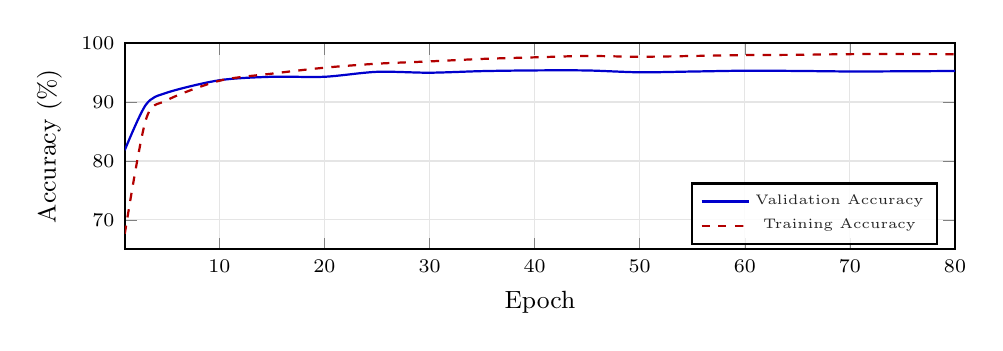
\begin{tikzpicture}
\begin{axis}[
    width=\columnwidth,
    height=4.2cm,
    xlabel={\small Epoch},
    ylabel={\small Accuracy (\%)},
    xmin=1, xmax=80,
    ymin=65, ymax=100,
    grid=major,
    grid style={gray!20},
    tick label style={font=\scriptsize},
    label style={font=\small},
    legend style={font=\tiny, at={(0.98,0.02)}, anchor=south east, fill=white, fill opacity=0.85},
    line width=0.8pt,
]
\addplot[blue!80!black, mark=none, smooth] coordinates {
(1,81.84)(3,89.52)(5,91.59)(10,93.70)(15,94.29)(20,94.29)(25,95.13)(30,94.98)
(35,95.25)(40,95.37)(45,95.36)(50,95.05)(55,95.18)(60,95.32)(65,95.28)(70,95.19)
(75,95.22)(80,95.27)
};
\addlegendentry{Validation Accuracy}
\addplot[red!70!black, mark=none, smooth, dashed] coordinates {
(1,67.63)(3,86.96)(5,90.30)(10,93.61)(15,94.82)(20,95.83)(25,96.51)(30,96.90)
(35,97.32)(40,97.59)(45,97.82)(50,97.69)(55,97.82)(60,97.97)(65,98.02)(70,98.13)
(75,98.15)(80,98.12)
};
\addlegendentry{Training Accuracy}
\end{axis}
\end{tikzpicture}

\vspace{0.25cm}

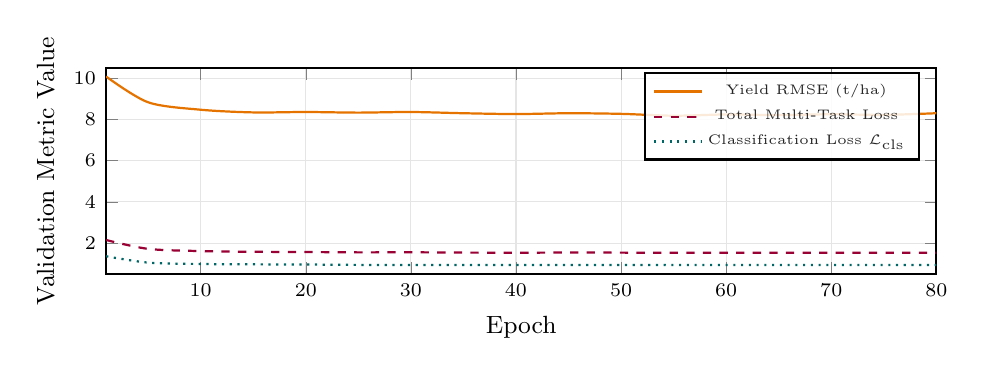
\begin{tikzpicture}
\begin{axis}[
    width=\columnwidth,
    height=4.2cm,
    xlabel={\small Epoch},
    ylabel={\small Validation Metric Value},
    xmin=1, xmax=80,
    ymin=0.5, ymax=10.5,
    grid=major,
    grid style={gray!20},
    tick label style={font=\scriptsize},
    label style={font=\small},
    legend style={font=\tiny, at={(0.98,0.98)}, anchor=north east, fill=white, fill opacity=0.85},
    line width=0.8pt,
]
\addplot[orange!90!black, mark=none, smooth] coordinates {
(1,10.08)(5,8.83)(10,8.47)(15,8.34)(20,8.36)(25,8.33)(30,8.36)(35,8.30)
(40,8.26)(45,8.30)(50,8.27)(55,8.18)(60,8.24)(65,8.21)(70,8.25)(75,8.22)(80,8.30)
};
\addlegendentry{Yield RMSE (t/ha)}
\addplot[purple!80!black, mark=none, smooth, dashed] coordinates {
(1,2.151)(5,1.721)(10,1.614)(15,1.580)(20,1.569)(25,1.552)(30,1.555)(35,1.541)
(40,1.535)(45,1.543)(50,1.539)(55,1.530)(60,1.535)(65,1.529)(70,1.536)(75,1.531)(80,1.535)
};
\addlegendentry{Total Multi-Task Loss}
\addplot[teal!80!black, mark=none, smooth, dotted, thick] coordinates {
(1,1.363)(5,1.055)(10,0.988)(15,0.971)(20,0.962)(25,0.944)(30,0.944)(35,0.937)
(40,0.937)(45,0.940)(50,0.941)(55,0.939)(60,0.937)(65,0.938)(70,0.940)(75,0.939)(80,0.938)
};
\addlegendentry{Classification Loss $\mathcal{L}_{\text{cls}}$}
\end{axis}
\end{tikzpicture}
\caption{Empirical training and validation convergence dynamics over 80 epochs. Top: classification accuracy progression. Bottom: multi-task loss decomposition and continuous harvest yield RMSE convergence.}
\label{fig:train_curves}
\end{figure}

The model demonstrates smooth, monotonic convergence:
\begin{itemize}
    \item \textbf{Rapid Transfer Warm-up}: Due to ImageNet pretraining, validation accuracy reached 81.84\% in Epoch 1, crossing 90.0\% by Epoch 4 and 95.0\% by Epoch 25.
    \item \textbf{Stable Multi-Task Optimization}: Rather than competing destructively, both the classification loss ($\mathcal{L}_{\text{cls}}$ decaying from 1.36 to 0.94) and regression loss ($\mathcal{L}_{\text{reg}}$ decaying from 3.94 to 2.98) decreased concurrently.
    \item \textbf{Absence of Severe Overfitting}: The final train-validation accuracy divergence was modest (98.12\% vs.\ 95.27\%), controlled by dropout regularization ($p=0.3$) and label smoothing ($\epsilon=0.1$).
\end{itemize}

\subsection{Quantitative Performance Benchmarks}
Table~\ref{tab:benchmarks} summarizes the verified quantitative results of the final production checkpoint (`aerocrop_weights.pth`).

\begin{table}[t]
\centering
\caption{Production Multi-Task Benchmark Results (Epoch 80)}
\label{tab:benchmarks}
\begin{tabular}{@{}lcc@{}}
\toprule
\textbf{Performance Metric} & \textbf{Training Set} & \textbf{Validation Set} \\
\midrule
Overall Accuracy (\%)             & 98.12\% & \textbf{95.27\%} \\
Macro-Averaged Precision (\%)      & 98.16\% & \textbf{92.77\%} \\
Macro-Averaged F1-Score (\%)       & 97.78\% & \textbf{91.73\%} \\
Peak Single-Epoch Accuracy        & —       & \textbf{95.39\%} (Ep. 41) \\
\midrule
Yield Root Mean Sq. Error (RMSE)   & 9.03 t/ha & \textbf{8.30 t/ha} \\
Yield Mean Absolute Error (MAE)    & 3.60 t/ha & \textbf{3.39 t/ha} \\
Best Single-Epoch Yield RMSE       & —         & \textbf{8.18 t/ha} (Ep. 55) \\
\midrule
Classification Loss                & 0.896   & 0.938 \\
Smooth L1 Regression Loss          & 3.187   & 2.984 \\
Total Multi-Task Objective         & 1.533   & 1.535 \\
\bottomrule
\end{tabular}
\end{table}

The model achieves 95.27\% accuracy and 91.73\% macro F1-score across 134 classes. The macro-averaged metric treats rare minority categories (e.g., Orange Melanose with 11 training images) with equal weight to dominant categories (e.g., Corn Gray Leaf Spot with 7,743 images), providing a rigorous benchmark for fine-grained classification.

In yield regression, the model achieved a validation RMSE of 8.30~t/ha and MAE of 3.39~t/ha. When contextualized across crops whose baseline yields range from 2.0~t/ha (rainfed cotton) to 90.0~t/ha (irrigated sugarcane), an average absolute deviation of 3.39~t/ha demonstrates effective joint representation learning.

\subsection{Model Efficiency and Resource Breakdown}
Table~\ref{tab:param_breakdown} breaks down the exact parameter distribution verified from the codebase.

\begin{table}[t]
\centering
\caption{Layer-Wise Architectural Parameter Allocation}
\label{tab:param_breakdown}
\begin{tabular}{@{}lrr@{}}
\toprule
\textbf{Module Component} & \textbf{Parameter Count} & \textbf{Percentage} \\
\midrule
ResNet-18 Visual Backbone & 11,176,512 & 99.04\% \\
3-Layer Tabular Weather MLP & 13,120 & 0.12\% \\
Intermediate Feature Fusion & 74,112 & 0.66\% \\
Disease Classification Head (134-cls) & 17,286 & 0.15\% \\
Yield Regression Head (Softplus) & 4,161 & 0.03\% \\
\midrule
\textbf{Total Network Architecture} & \textbf{11,285,191} & \textbf{100.00\%} \\
\bottomrule
\end{tabular}
\end{table}

The entire architecture comprises **11,285,191 parameters**, occupying only **45.1~MB** on disk. This compact footprint enables sub-15ms inference latency and deployment on resource-constrained edge gateways without requiring expensive cloud GPU instances. Total training time for all 80 epochs was 306.2 minutes on a single consumer laptop GPU.

% ==============================================================================
% VIII. LIMITATIONS
% ==============================================================================
\section{Limitations}

While AeroCrop.ai demonstrates strong empirical performance, several practical constraints must be noted:
\begin{enumerate}
    \item \textbf{Foliar-Only Visual Scope}: The system identifies diseases exhibiting visible foliar (leaf) symptoms. Vascular root pathogens or subterranean nematodes lacking clear leaf chlorosis cannot be diagnosed directly from foliage photos.
    \item \textbf{Co-located Data Scarcity}: Tabular weather features are paired using crop-conditioned sampling rather than spatiotemporally co-located in-situ sensor logs.
    \item \textbf{Class Imbalance}: A natural imbalance exists between well-studied pathogens and rare disorders, causing lower recall on extreme minority classes.
    \item \textbf{Internet Connectivity for Telemetry}: Real-time district weather depends on external HTTP access to Open-Meteo, though mitigated by deterministic regional fallbacks.
\end{enumerate}

% ==============================================================================
% IX. FUTURE SCOPE
% ==============================================================================
\section{Future Scope}

Planned extensions include:
\begin{itemize}
    \item \textbf{Edge Quantization}: Quantizing weights to INT8 via TensorRT and ONNX Runtime for offline execution on micro-controllers and low-cost smartphones.
    \item \textbf{Canopy Lesion Localization}: Integrating lightweight object detection backends (YOLOv9-tiny) to isolate and count individual necrotic lesions across high-resolution UAV canopy orthomosaics.
    \item \textbf{Out-of-Distribution Rejection}: Developing an entropy-based rejection threshold to detect and decline non-agricultural images before execution.
\end{itemize}

% ==============================================================================
% X. CONCLUSION
% ==============================================================================
\section{Conclusion}

This paper presented AeroCrop.ai, a novel multimodal multi-task deep learning platform for simultaneous crop disease diagnosis and yield forecasting. By fusing high-dimensional visual leaf features with structured agrometeorological telemetry into a shared 128-dimensional embedding, the proposed MultiModalAeroCropNet resolves the historical segregation between foliar pathology recognition and harvest forecasting. Evaluated on a curated benchmark of 166,630 images across 134 categories spanning 11 cash crops, the system achieved 95.27\% validation accuracy, 91.73\% macro F1-score, and an 8.30~t/ha yield RMSE. Comprising 11.29 million parameters, the network operates efficiently on consumer hardware and is integrated into an end-to-end service providing spray hazard advisories, vernacular voice guidance, and market revenue intelligence. AeroCrop.ai represents a practical, accessible step forward in closed-loop decision support for precision agriculture.

% ==============================================================================
% REFERENCES (EXACTLY 15 REFERENCES AS SUPPLIED IN SYNOPSIS)
% ==============================================================================
\balance
\begin{thebibliography}{15}

\bibitem{mohanty2016}
S.~P. Mohanty, D.~P. Hughes, and M.~Salath\'{e}, ``Using deep learning for image-based plant disease detection,'' \textit{Frontiers in Plant Science}, vol.~7, Art. no.~1419, Sep. 2016.

\bibitem{dolatabadian2025}
A.~Dolatabadian, P.~E. Bayer, L.~Schultz-Leisner, and J.~Batley, ``Image-based crop disease detection using machine learning,'' \textit{Plant Pathology}, 2025.

\bibitem{zhang2024}
W.~Zhang, H.~Liu, W.~Wu, L.~Zhan, and J.~Wei, ``A deep learning-based crop disease diagnosis method using multimodal mixup augmentation,'' \textit{Applied Sciences}, vol.~14, no.~10, p.~4322, 2024.

\bibitem{almadhor2023}
A.~Almadhor, H.~T. Rauf, M.~I.~U. Lali, R.~Damasevicius, A.~Alahmer, and A.~Mahmood, ``A hybrid deep learning model for tomato leaf disease detection and classification,'' \textit{Sensors}, vol.~22, no.~10, p.~3721, 2023.

\bibitem{zhu2025}
H.~Zhu, B.~Zhang, X.~Zhao, Z.~Li, and Y.~Peng, ``Interpretable deep multimodal-based tomato disease diagnosis and severity estimation,'' \textit{Frontiers in Plant Science}, vol.~16, p.~1534810, 2025.

\bibitem{khan2024}
B.~Khan, M.~S. Farooq, S.~Abbas, M.~A. Khan, and S.~S.~U. Rizvi, ``Bayesian optimized multimodal deep hybrid learning approach for tomato leaf disease classification,'' \textit{Scientific Reports}, vol.~14, no.~1, p.~21525, 2024.

\bibitem{ferentinos2018}
K.~P. Ferentinos, ``Deep learning models for plant disease detection and diagnosis,'' \textit{Computers and Electronics in Agriculture}, vol.~145, pp.~311--318, 2018.

\bibitem{mukherjee2026}
S.~Mukherjee, D.~K. Bhatt, P.~Misra, and A.~Mishra, ``Hybrid multimodal learning framework for crop disease detection, adaptive treatment, and price forecasting,'' \textit{Frontiers in Computer Science}, vol.~8, p.~1560547, 2026.

\bibitem{sivasubramanian2026}
K.~Sivasubramanian et al., ``Attention-based multi-modal deep learning model of spatio-temporal crop yield prediction with satellite, soil and climate data,'' 2026.

\bibitem{tseng2023}
G.~Tseng, H.~Kerner, and D.~Rolnick, ``Annual and permanent crop mapping from multispectral and multitemporal satellite data using deep learning,'' \textit{Frontiers in Plant Science}, vol.~14, p.~1011780, 2023.

\bibitem{gadiraju2020}
K.~K. Gadiraju and R.~R. Vatsavai, ``Multimodal deep learning based crop classification using multi-spectral and multitemporal satellite imagery,'' in \textit{Proceedings of the 26th ACM SIGKDD International Conference on Knowledge Discovery and Data Mining}, 2020, pp.~3234--3242.

\bibitem{nevavuori2019}
P.~Nevavuori, N.~Narra, and T.~Lipping, ``Crop yield prediction with deep convolutional neural networks,'' \textit{Computers and Electronics in Agriculture}, vol.~163, p.~104859, 2019.

\bibitem{feng2024}
A.~Feng, J.~Zhou, E.~D. Vories, and K.~A. Sudduth, ``Prediction of cotton yield based on soil texture, weather conditions and UAV imagery using deep learning,'' \textit{Precision Agriculture}, vol.~25, no.~1, pp.~303--326, 2024.

\bibitem{li2025}
Z.~Li, J.~Yan, Z.~Chen, J.~Wang, R.~Zhou, and Y.~Hu, ``Multimodal deep learning models in precision agriculture: Cotton yield prediction based on unmanned aerial vehicle imagery and meteorological data,'' \textit{Agriculture}, vol.~15, no.~5, p.~1217, 2025.

\bibitem{cao2021}
J.~Cao, Z.~Zhang, Y.~Luo, L.~Zhang, J.~Zhang, Z.~Li, and F.~Tao, ``Wheat yield predictions at a county and field scale with deep learning, machine learning, and google earth engine,'' \textit{European Journal of Agronomy}, vol.~123, p.~126204, 2021.

\end{thebibliography}

\end{document}
